\documentclass[../mit-general-chemistry.tex]{subfiles}
\begin{document}

\chapter{Energies and enthalpies of chemical reactions}



Considering a chemical reaction

\ceeqstar{CH4 -> CH3 + H}

We remind ourselves of the concept of {\em bond (dissociation) energy}
and that that is the energy required to break some covalent bond.


The related concept of {\em bond enthalpy} ($\Delta H$) is the heat
associated with the dissociation of a bond (meassured under constant
pressure).

Enthalpy is closely related to energy through the relation seen in
\begin{equation}\label{eq:enthalpy}
  \Delta H = \Delta E + \Delta(PV)
\end{equation}

Enthalpy (Symbol: $H$) is a measurement of energy in a thermodynamic
system. It is the thermodynamic quantity equivalent to the total heat
content of a system. It is equal to the internal energy of the system
plus the product of pressure and volume.

Consider a process carried out at constant pressure and where the only
allowed {\em work} is pressure-volume work (no lifting, dropping or
otherwise adding of energy) $w = -P\Delta V$. Then
\begin{equation}\label{eq:heatconstantpressure}
  \Delta E = q_P + w
  \implies
  \Delta E = q_P - P\Delta V
  \Leftrightarrow
  q_P = \Delta E + P\Delta V
\end{equation}
for $q_P$, the {\em heat} at constant pressure.

Now, for our system, at constant pressure, Equation~\ref{eq:enthalpy}
and Equation~\ref{eq:heatconstantpressure} allow us to claim that

\begin{equation*}
  \enthalpy = \Delta E + P\Delta V = q_P
\end{equation*}


For gasses, $\Delta H$ and $\Delta E$ differ only by one to two
percent. For solids the difference between $\Delta H$ and $\Delta E$
is going to be negligible. For this reason we are going to focus on
bond enthalpy in this discussion.

Contrary to bond energy, bond enthalpy is easily measured.

For a chemical reaction
\begin{equation*}
  \enthalpy_r = H_{\text{products}} - H_{\text{reactants}}
\end{equation*}


When chemical bonds are broken, the energy of those bonds is released
by a system and as bonds are formed energy is absorbed from the
system.

{\em Standard bond enthalpy} (\stdbondenthalpy) is the known enthalpy
for a specific bond at room temperature, \SI{298}{\kelvin} with the
elements being in their {\em natural state}. If we are concerned with
gasses, the standard bond enthalpy refers to conditions under standard
air pressure, possibly \SI{1}{\bar}.

$\Delta H$ is a positive change in endothermic reactions, and negative
in heat-releasing exothermic processes.




Let's compare \stdbondenthalpy for some different carbon-hydrogen
bonds, all in gaseous states.

\begin{align*}
  &\ce{CH4 -> CH3 + H} &\stdbondenthalpy = + \SI{438}{\kilo\joule\per\mol} \\
  &\ce{C2H6 -> C2H5 + H} &\stdbondenthalpy = + \SI{410}{\kilo\joule\per\mol} \\
  &\ce{CHF3 -> CF3 + H} &\stdbondenthalpy = + \SI{429}{\kilo\joule\per\mol} \\
  &\ce{CHCl3 -> CCl3 + H} &\stdbondenthalpy = + \SI{380}{\kilo\joule\per\mol} \\
  &\ce{CHBr3 -> CBr3 + H} &\stdbondenthalpy = + \SI{377}{\kilo\joule\per\mol} \\
\end{align*}

The fact that $\stdbondenthalpy > 0$ in these cases means that we
would need to put in energy to break that bond, that the reaction is
{\em endothermic}.

The overview shows that \stdbondenthalpy depends on even the context
of the bond, what other bonds of the carbon atom.

It is worth noting that the enthalpies of the listed carbon-hydrogen
bonds all lie within 8\% of the average value (412 \kjpm). It is
common to list and use {\em the average enthalpy}
($\mean{\stdbondenthalpy}$ or $\mean{\enthalpy}$) for bonds involving
the elements (i.e. average carbon-hydrogen bond enthalpy is 412
\kjpm).

The difference between bond enthalpies in products and reactants gives
an estimate of the enthalpy of the reaction.

Let's do that. The reaction we will consider is the oxidation of glucose.

\begin{align*}
  &\ce{C6H12O6 + 6O2 -> 6CO2 + 6H2O} &\stdbondenthalpy_r = -2816 \kjpm
\end{align*}

We conclude, since $\stdbondenthalpy < 0$, that this is an exothermic
reaction -- it will give off heat.


The oxidation of glucose is the major source of energy for all
animals. It is going on all the time in our bodies.

Plants do the reverse.
\begin{align*}
  \ce{6CO2 + 6H2O &->[\text{sun light}] 6O2 + C6H12O6} &\text{(photosynthesis)}
\end{align*}
We know that this is going to take energy and the plants take this
energy from the sun.

When we eventually eat plants or animals that have eaten plants we
can harness the stored energy.



In the breakdown of glucose and oxygen, we are not really concerned
with the products of the reaction, instead we store the
$\stdbondenthalpy_r = -2816 \kjpm$ in the form of ATP, the currency of
energy in the cell.

To calculate the enthalpy of a reaction, we calculate
\begin{equation*}
  \stdbondenthalpy_r = \sum \Delta H_i - \sum \Delta H_j
\end{equation*}
where $H_i$ is the bond enthalpy for all the reactants and $H_j$ is
the enthalpy of all the products.

If the bonds of the products are stronger than the bonds of the
reactants then $\stdbondenthalpy_r < 0$ and we know that this means
that the reaction is exothermic.

If the bonds of the reactants are stronger than the bonds of the
products then $\stdbondenthalpy_r > 0$ which tells us that the
reaction is endothermic.

So let's be explicit about the reaction. We have
\ceeqstar{C6H12O6 + 6O2 -> 6CO2 + H2O}

with the following structural formulas for each compound.

\begin{center}
  \chemname{\chemfig{C(=[:135]O)(-[:225]H)-C(-[:90]O-[:90]H)(-[:270]H)-C(-[:90]O-[:90]H)(-[:270]H)-C(-[:90]O-[:90]H)(-[:270]H)-C(-[:90]O-[:90]H)(-[:270]H)-C(-[:90]O-[:90]H)(-[:270]H)-H}}{glucose}
\end{center}

\hspace*{\fill}
\chemname{\chemfig{O=O}}{oxygen gas}
\hfill
\chemname{\chemfig{O=C=O}}{carbon dioxide}
\hfill
\chemname{\chemfig{\lewis{1:3:,O}(-[:218]H)(-[:322]H)}}{water}
\hspace*{\fill}


Now, we can count the number of bonds of each type

\begin{center}
  \begin{tabular}{llll}
    \toprule
    Bond type & Reactants & Products & $\mean{\enthalpy}$ \\
    & & &  {\small (\kjpm)} \\
    \midrule
    \chemfig{C-H} & 7 &   & 414 \\
    \chemfig{C-C} & 5 &   & 368 \\
    \chemfig{C-O} & 5 &   & 352 \\
    \chemfig{C=O} & 1 & 12 & 532 \\
    \chemfig{O-H} & 5 & 12 & 465 \\
    \chemfig{O=O} & 6 & & 498 \\
    \bottomrule
  \end{tabular}
\end{center}


Now we can calculate the enthalpy for the reactants and the products
in the reaction.
\begin{align*}
  \sum \enthalpy_r =~&(7\times 414) + (5\times 368) + (5\times 352) + (5\times 465) +\\
  &+ (1\times 532) + (6\times 498)~\kjpm =  12343~\kjpm \\
  \sum \enthalpy_p =~&(12\times 465) + (12\times 532)~\kjpm =  11964~\kjpm \\
\end{align*}

{\color{red}\textbf{Kolla det här! Siffrorna skall bli $12452 - 15192
    = -2740$~\kjpm}}

The difference between the change of enthalpy between the reactants on
one side and the products on the other is then
\begin{equation*}
  \stdbondenthalpy_r = 12343 - 11964~\kjpm = ~\kjpm
\end{equation*}


From the numbers of the MIT lecture we see that the numbers are
similar but not the same ($2740 \neq 2816$) but the difference is
within 3\% and that is pretty good. Remeber that we're not using exact
bond enthalpies here but the mean bond enthalpies. So we know we're
going to be somewhat off.




\subsubsection{Heat of formation}

Another way of thinking about the total heat of reactions is through
the concept of {\em heat of formation} ($\Delta H_f^0 = \Delta H_r^0$)
of a reaction forming \SI{1}{\mol} of compund from pure elements in
their most stable form at standard state, that is $P = \SI{1}{\bar}$
and $T = \SI{298}{\kelvin}$.

For instance, let's consider the formation of water. It is made out of
hydrogen, which in it's most stabl form at $P = \SI{1}{\bar}$ and $T =
\SI{298}{\kelvin}$ is in the form of hydrogen gas \ce{H2}. Water also
conatins oxygen , which in it's most stabl form at $P = \SI{1}{\bar}$
and $T = \SI{298}{\kelvin}$ is in the form of oxygen gas, \ce{O2}. The
reaction of formation of water can be summarized as
\begin{multline*}
  \ce{H2(g) + \sfrac{1}{2} O2(g) -> H2O} \\
  \Delta H^0 = -285.83~\kjpm = \Delta H_f^0~\text{for \ce{H2O}}
\end{multline*}
Similarly we can look up the heat of formation of carbon dioxide out
of ground up carbon (it's stable state at $P = \SI{1}{\bar}$ and $T =
\SI{298}{\kelvin}$) and oxygen gas.
\begin{multline*}
  \ce{C_{gr} + O2(g) -> CO2(g)} \\
  \Delta H^0 = -393.5~\kjpm = \Delta H_f^0~\text{for \ce{CO2(g)}}
\end{multline*}
The $H_f^0$ for an element in it's most stable state is zero.

For instance
\begin{align*}
  &\ce{O2(g) -> O2(g)}
  &\Delta H^0 = 0~\kjpm = \Delta H_f^0~\text{for \ce{O2(g)}} \\
\end{align*}
The heat of formation of one mole of glucose is
\begin{multline*}
  \ce{3O2(g) + 6C_{gr} + 6H2(g) -> C6H12O6} \\
  \Delta H^0 = -1260~\kjpm = \Delta H_f^0~\text{for \ce{C6H12O6}} \\
\end{multline*}


Now, let's see if we can do any better with approximate the heat from
oxidation of glucose, using heat of formation for estimations of bond
enthalpy.

First, we display the structures of reactants and products of
oxidation of glucose.
\begin{center}
  \chemname{\chemfig{C(=[:135]O)(-[:225]H)-C(-[:90]O-[:90]H)(-[:270]H)-C(-[:90]O-[:90]H)(-[:270]H)-C(-[:90]O-[:90]H)(-[:270]H)-C(-[:90]O-[:90]H)(-[:270]H)-C(-[:90]O-[:90]H)(-[:270]H)-H}}{glucose}
\end{center}

\hspace*{\fill}
\chemname{\chemfig{O=O}}{oxygen gas}
\hfill
\chemname{\chemfig{O=C=O}}{carbon dioxide}
\hfill
\chemname{\chemfig{\lewis{1:3:,O}(-[:218]H)(-[:322]H)}}{water}
\hspace*{\fill}

From these structural formulas and the different values we can look up
for the heat (enthalpy) of formation for the different compounds, we
can calculate the enthalpy for this reaction we calculate
\begin{align*}
  \Delta H_r^0 = &\ce{[6\Delta H_f^0(CO2)] + [6\Delta H_f^0(H2O)]} - \\
  &- (\ce{[6\Delta H_f^0(O2)] + [\Delta H_f^0(C6H12=6)]}) = \\
  &= 6(-393.5) + 6(-285.8) - 1(-1260) - 0 = \\ &
  = -2827.8~\kjpm~\text{of}~\ce{C6H12O6} \\
  &{\color{red} -2816~\kjpm}
\end{align*}

And from the MIT lecture we see that $\Delta H_r^0{}_{calculated} =
\Delta H_r^0{}_{experimental} = -2816~\kjpm$.


There is actually one more way to figure out $\Delta H_r^0$ for a
reaction.



\subsubsection{Hess' law}



We recognize that {\em enthalpy is a state function}. That is,
\enthalpy is independent of path. Like altitude which is independent
of the way you take to get to some point. Whether you climb straight
up to a point on a mountain side or you go up to the top before
landing on the point, you're altitude will be the same.

This means you're able to use known values of $\Delta H_r^0$ for
different reactions and sum up and subtract these values to calculate
the differences of $\Delta H_r^0$ of two compounds that can be found
going through a path leading from the initial compound to the final.


\begin{definition}[Hess' Law]
  If two or more chemical equations are added to give another chemical
  equation we mist add the corresponding enthalpy.

  This is in reference to calculating enthalpy of a reaction.
\end{definition}


Using Hess' law we can find the enthalpy for a reaction by adding and
subtracting known values of $\enthalpy_f$ for reactions that form a
path from the reaction's reactants to it's products.

\begin{figure}[t]
  \begin{margincap}
    \begin{center}
      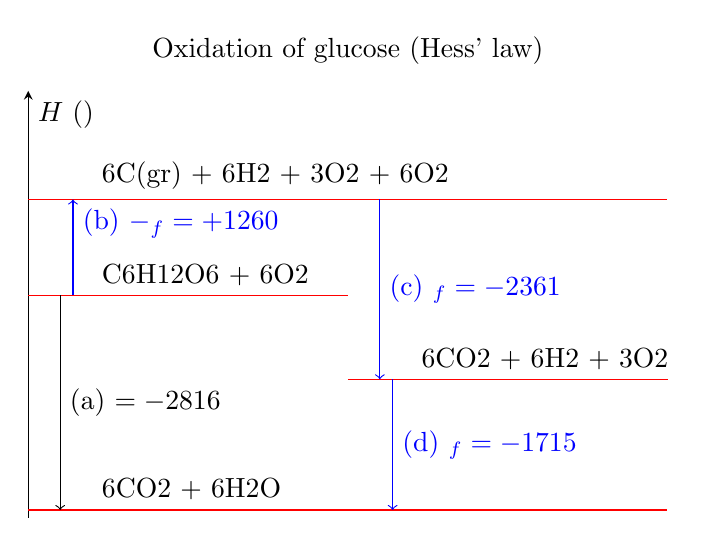
\begin{tikzpicture}
        \begin{axis}[
            title={Oxidation of glucose (Hess' law)},
            ylabel={$H$ (\kjpm)},
            width=.8\textwidth,
            height=7cm,
            axis lines = middle,
            hide x axis,
            domain = 0:10,
            ymin=-100,
            ymax=5500,
            xmin=0,
            xmax=10,
            ytick =\empty,
            clip = false,
            every axis plot post/.append style={red,mark=none}
          ]
          \addplot[domain=0:10]{0};
          \node at (axis cs:1,0) [anchor=south west] {\ce{6CO2 + 6H2O}};
          
          \addplot[domain=0:5]{2816};
          \node at (axis cs:1,2816) [anchor=south west] {\ce{C6H12O6 + 6O2}};
          
          \addplot[domain=0:10]{4076};
          \node at (axis cs:1,4076) [anchor=south west] {\ce{6C(gr) + 6H2 + 3O2 + 6O2}};
          
          \addplot[domain=5:10]{1715};
          \node at (axis cs:6,1715) [anchor=south west] {\ce{6CO2 + 6H2 +
              3O2}};
          
          \draw[->] (axis cs:0.5, 2816) -- (axis cs:0.5, 0)
          node[midway,right]{(a) $\enthalpy = -2816~\kjpm$};
          
          \draw[->,blue] (axis cs:0.7, 2816) -- (axis cs:0.7, 4076)
          node[pos=.75,right]{(b) $-\enthalpy_f = +1260~\kjpm$};
          
          \draw[->,blue] (axis cs:5.5, 4076) -- (axis cs:5.5, 1715)
          node[midway,right]{(c) $\enthalpy_f = -2361~\kjpm$};
          
          \draw[->,blue] (axis cs:5.7, 1715) -- (axis cs:5.7, 0)
          node[midway,right]{(d) $\enthalpy_f = -1715~\kjpm$};
        \end{axis}
      \end{tikzpicture}%
    \end{center}
  \caption{Since enthalpy is a state function we are just interested
    in the final energy difference, not the path. In the diagram, (a)
    oxidation of glucose; (b) decomposition of glucose into it's
    elements; (c) formation of \ce{CO2}; (d) formation of \ce{H2O}.
  \label{fig:hesslaw}}
  \end{margincap}
\end{figure}

This means that if we are calculating $\Delta H_r^0$ for
\ceeqstar{C6H12O6 + 6O2 -> 6CO2 + 6H2O}
we can calculate it from

\begin{align*}
  &\ce{C6H12O6 + 6O2 -> 6C(gr) + 6H2(g) + 3O2 + 6O2} \\
  &\qquad-\Delta H_f^{\circ} = +1260~\kjpm \\
  &\ce{6C(gr) + 6H2(g) + 3O2 + 6O2 -> 6CO2 + 6H2 + 3O2} \\
  &\qquad\Delta H_f^{\circ} = -2361~\kjpm \\
  &\ce{6CO2 + 6H2 + 3O2 -> 6CO2 + 6H2O} \\
  &\qquad\Delta H_f^{\circ} = -1715~\kjpm \\
\end{align*}

Which gives us a total of

\begin{align*}
  &\ce{C6H12O6 + 6O2 -> 6CO2 + 6H2O} \\
  &\qquad\Delta H_r^0 = \sum\Delta H_f^{\circ} = -2816~\kjpm \\
\end{align*}

Which we know it to be. Another depiction of this approach can be seen
in Fig.~\ref{fig:hesslaw}. Again, Hess' law works since enthalpy is a
state function.




\addsec{Summary}

The {\em enthalpy} of a reaction ($\enthalpy_r$) is the energy, heat,
needed for the reaction to occur (endothermic reaction) or released
during the reaction (exothermic reaction).

A reaction have a left hand side (reactants) and a right hand side
(products). As the reaction progresses (to the right) the bonds of the
reactants are broken and new bonds of the products are formed.

We have covered three ways to calculate the enthalpy of a given
reaction, $\enthalpy_r$.

We can use average bond enthalpy (\enthalpy without subscript or
$\enthalpy_B$). To use these values of enthalpy we calculate the sum
of the bonds that are broken among the reactants and subtract the sum
of the bonds that are formed among the products.
\begin{equation}\label{eq:sum:bondenthalpy}
  \enthalpy_r = \sum \enthalpy_B(\text{reactants}) - \sum \enthalpy_B(\text{products})
\end{equation}

We can also use {\em enthalpy of formation} ($\enthalpy_f$). Enthalpy
of formation or {\em heat of formation} is the energy it takes to form
a given molecule.

To calculate the enthalpy of some reaction we calculate the difference
between the enthalpy of formation of the products and the enthalpy of
formation of all of the reactants.
\begin{equation}\label{eq:sum:enthalpyofformation}
  \enthalpy_r = \sum \enthalpy_f(\text{products}) - \sum \enthalpy_f(\text{reactants})
\end{equation}

We see that the order of the reactants and products in
Equation~\ref{eq:sum:bondenthalpy} and
Equation~\ref{eq:sum:enthalpyofformation} are different. This is
because of the energies we use for the calculations is different. When
we refer to bond enthalpy, this is energy that is release from broken
bonds and absorbed by formed bonds. When we refer to enthalpy of
formation we must remember that the bonds of the reactants are going
to be broken and that this gives us a negative number for the
reactants and a positive number for the products. So the signs of the
terms are shifted between the two equations.


Hess' law claims that since enthalpy is a {\em state function}, the
internal energy of a system in a final state of a chemical reaction is
the same, however this state is reached. As we saw in the examples of
this chapter, we can use known values of bond enthalpy or enthalpy of
formation of other reactions that also could lead up to the products
of our reaction and find $\enthalpy_r$ by arithmetic operations.






\end{document}
